\documentclass[10pt,t]{beamer}
\usetheme{Heverlee}

\usepackage{tikz-cd}

\newcommand{\F}{\mathbb F}


%%% QUICK OPTIONS:
% (A) Math font without serifs, enable line below to make math serif:
    \usefonttheme[onlymath]{serif}

% (B) Re-define primary colour by adjusting the RGB values
    %\definecolor{pblue}	{RGB}{206,125,66}

% (C) Title page graphic (optional) --- this is not for the background image, see \usebackgroundtemplate to change that ---
    %\titlegraphic{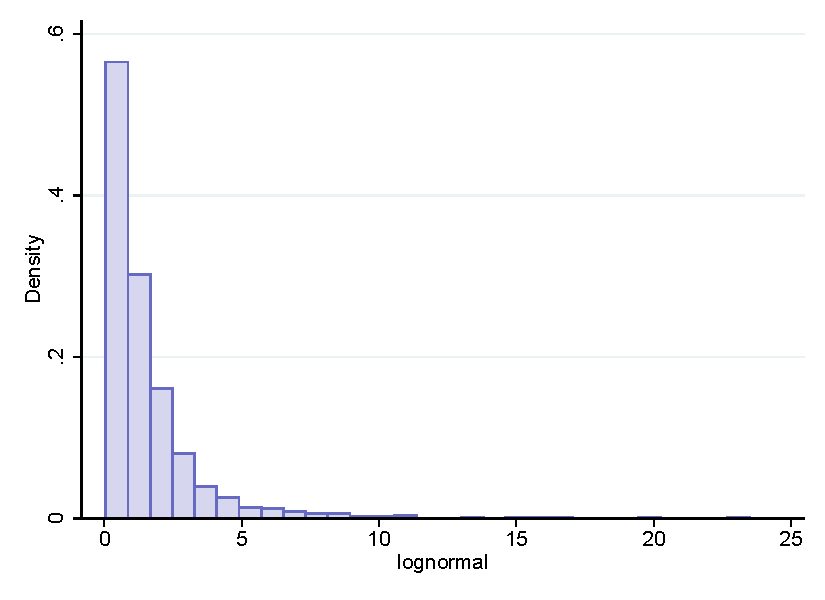
\includegraphics[height=2.7cm]{example_figure.pdf}}

% (D) Add logo to bottom right-corner (optional)
    \logo{
\includegraphics[height=0.7cm]{logo.png}\hspace{12pt}\vspace{-6pt}}      

% (E) Choose one (or none) of these lines to add footline bar on all frames
    %\setbeamertemplate{footline}[infoline]  % author, title, insitute
    %\setbeamertemplate{footline}[navigation] % dots swhowing progress
    %\setbeamertemplate{footline}[navsym] % navigation symbols

% (F) Widescreen 16:9 ratio
    %\usepackage[orientation=landscape,size=custom,width=16,height=9,scale=0.45,debug]{beamerposter} 



%%% TITLE PAGE INFO:

\title[clesto]{Chain level Steenrod operations}
\subtitle{Theoretical and computational aspects}
\author[ammedmar]{Anibal M. Medina-Mardones}
\institute{Max Planck Institute for Mathematics in Bonn}
\date{January 2021}

\begin{document}
% Title page

{
% Change image, or delete this line to remove background image
\usebackgroundtemplate{ \parbox[b][\paperheight][b]{\paperwidth}{\centering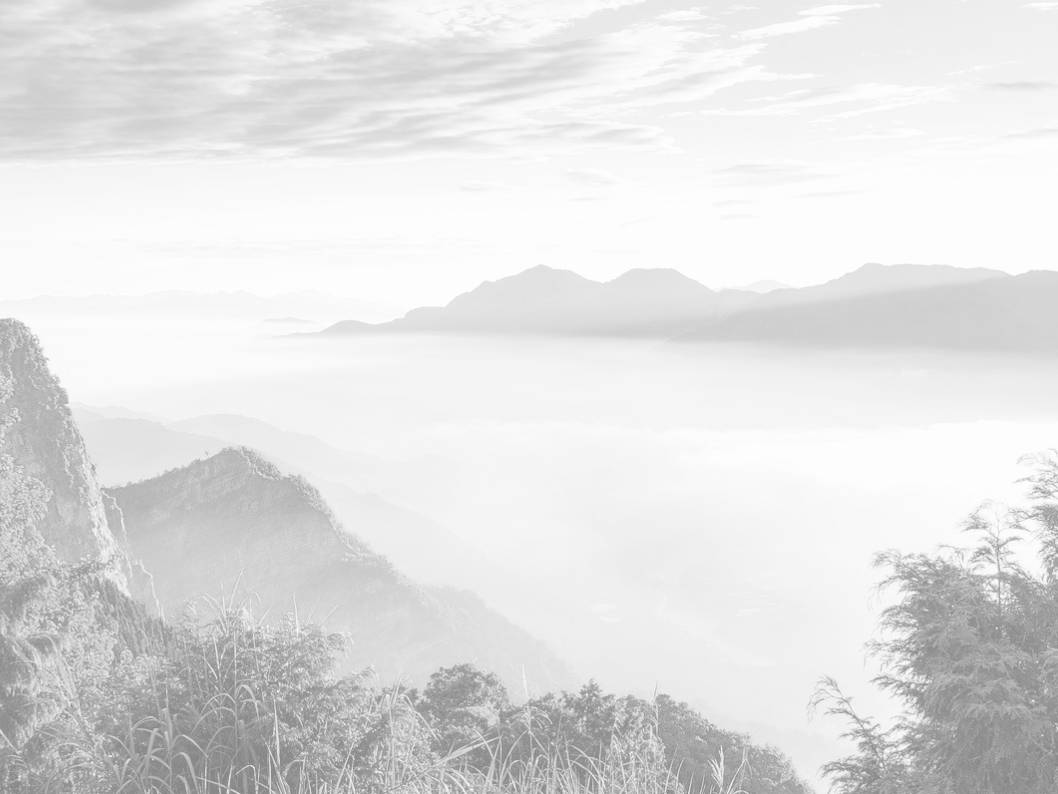
\includegraphics[width=\paperwidth]{bg_alishan.jpg}}} 
 %   abudhabi      cherry      forest      river
 %   alishan       chobe       leuven      sanfancisco
 %   blueprint     columns     library     uyuni
 %   bokeh         flowers     newyork     winter

% \setbeamercolor{background canvas}{bg=lgray}  % make background light gray

\begin{frame}[plain,noframenumbering]
    \titlepage
\end{frame}
}

% Table of contents slide
\begin{frame}{Outline}
	\vskip 2mm
	\hfill	{\large \parbox{.95\textwidth}{\tableofcontents[hideothersubsections]}}
\end{frame}

%%  SECTION 1

\section{History and motivation} \label{sec: history and motivation}

\begin{frame}[fragile]{Diagonal and cup product}
	The diagonal map of spaces
	\begin{equation*}
	\begin{tikzcd}[row sep = tiny]
	X \arrow[r, "D"] & X \times X \\
	x \arrow[r, |->]& (x, x)
	\end{tikzcd}
	\end{equation*}
	induces a product in cohomology 
	\begin{equation*}
	\begin{tikzcd}[row sep = tiny]
	H^\bullet \otimes H^\bullet \arrow[r, "\smallsmile"] & H^\bullet \\
	\end{tikzcd}
	\end{equation*}
	which is (graded) commutative, since the diagonal is invariant under the transposition
	\begin{equation*}
	\begin{tikzcd}[row sep = tiny]
	X \times X \arrow[r, "T"] & X \times X \\
	(x, y) \arrow[r, |->]& (y, x).
	\end{tikzcd}
	\end{equation*}
\end{frame}


\begin{frame}[fragile]{Diagonal and cup product}
	During the mid 1930's Alexander, Kolmogorov, \v{C}ech and Whitney lifted this product to the cochain level by dualizing a simplicial chain approximation to the diagonal map
	\begin{equation*}
	\begin{tikzcd}[%
	,row sep = 0ex
	,/tikz/column 1/.append style={anchor=base east}
	,/tikz/column 2/.append style={anchor=base west}
	]
	C_\bullet \arrow[r, "\Delta"] & C_\bullet \otimes C_\bullet \\
	{[0, \dots, n]} \arrow[r, |->] & \sum_{i=0}^{n} {[0, \dots, i] \otimes [i, \dots, n]}.
	\end{tikzcd}
	\end{equation*}

	\pause
		
	It is not invariant under the transposition
	\begin{equation*}
	\begin{tikzcd}[row sep = tiny]
	C_\bullet \otimes C_\bullet \arrow[r, "T"] & C_\bullet \otimes C_\bullet \\
	a \otimes b \arrow[r, |->]& (-1)^{|a||b|} b \otimes a,
	\end{tikzcd}
	\end{equation*}
	but, can it be made to be? \pause Over $\mathbb Q$, yes; over $\mathbb F_p$?
	
	\vspace*{10pt} \pause
	
	\textcolor{pblue}{Anachronism warning:} The map $\Delta$ was used to \textbf{define} the cup product. Functoriality wasn't yet fully developed.
\end{frame}


\begin{frame}{Steenrod's obstructions to commutativity}
	In 1947, Steenrod published his seminal paper introducing the square operations through an effective construction of homotopies correcting the lack of symmetry of $\Delta$ (denoted $\Delta_0 = $ from now on).
	
	\vspace*{15pt} \pause
	
	\textcolor{pblue}{Recall:} The set of linear maps between chain complexes is a chain complex. Furthermore, chain maps agree with $0$-cycles, and chain homotopies with $1$-boundaries.

	\vspace*{15pt}\pause
	
	\textcolor{pblue}{Notice:} The chain complex
	\begin{equation*} \label{eq: complex of maps to the tensor product}
	Hom\left(C_\bullet, C_\bullet^{\otimes 2}  \right)
	\end{equation*}
	has a right $\Sigma_2$-action induced from $T$, and there is a $0$-cycle of interest
	\begin{equation*}
	\Delta_0 - T \Delta_0.
	\end{equation*}
\end{frame}


\begin{frame}{Steenrod's obstructions to commutativity}
	The cup-$1$ coproduct
	\begin{equation*}
	\Delta_1 [0, \dots, n] = \sum_{i<j} \pm [0, \dots, i, j, \dots, n] \otimes [i, \dots, j]
	\end{equation*}
	is boundary killing this cycle. But is itself \textbf{not symmetric}.
	
	\vspace*{10pt} \pause
	
	Steenrod gave formulae for higher corrections, the cup-$i$ coproducts:
	\begin{equation*}
	\partial (\Delta_{i+1}) = \Delta_i - (-1)^i T \Delta_i.
	\end{equation*}
	
	\vspace*{0pt}\pause
	
	More abstractly, if
	\begin{equation*}
	W(2) \quad = \quad \mathbb Z[\Sigma_2] \stackrel{\ 1-T}{\longleftarrow} \mathbb Z[\Sigma_2] \stackrel{\ 1+T}{\longleftarrow} \mathbb Z[\Sigma_2] \stackrel{\ 1-T}{\longleftarrow} \cdots
	\end{equation*}
	is the minimal free resolution of $\mathbb Z$ as a $\mathbb Z[\Sigma_2]$-module, \pause he effectively constructed an equivariant chain map
	\begin{equation*}
	W(2) \otimes C_\bullet \to C_\bullet^{\otimes 2}.
	\end{equation*}
\end{frame}
	

\begin{frame}[fragile]{Steenrod obstructions to commutativity}
	Passing to orbits and $\F_2$-dualizing, we have a chain map between fix points
	\begin{equation*}
	\begin{tikzcd}
	Hom\left(C_\bullet \otimes C_\bullet, \F_2 \right)^{\Sigma_2} \arrow[r] &
	Hom\left(W(2) \otimes C_\bullet, \F_2 \right)^{\Sigma_2}
	\end{tikzcd}
	\end{equation*}
\end{frame}
%%%%%%%%%%%%%
\begin{frame}[fragile]{Steenrod obstructions to commutativity}
	Passing to orbits and $\F_2$-dualizing, we have a chain map between fix points
	\begin{equation*}
	\begin{tikzcd}
	Hom\left(C_\bullet \otimes C_\bullet, \F_2 \right)^{\Sigma_2} \arrow[r] &
	Hom\left(W(2) \otimes C_\bullet, \F_2 \right)^{\Sigma_2} \arrow[d] \\
	\left(C^\bullet \otimes C^\bullet\right)^{\Sigma_2} \arrow[u] &
	Hom\left(W(2)_{\Sigma_2} \otimes C_\bullet, \F_2 \right)
	\end{tikzcd}
	\end{equation*}
\end{frame}
%%%%%%%%%%%%%
\begin{frame}[fragile]{Steenrod obstructions to commutativity}
	Passing to orbits and $\F_2$-dualizing, we have a chain map between fix points
	\begin{equation*}
	\begin{tikzcd}
	Hom\left(C_\bullet \otimes C_\bullet, \F_2 \right)^{\Sigma_2} \arrow[r] &
	Hom\left(W(2) \otimes C_\bullet, \F_2 \right)^{\Sigma_2} \arrow[d] \\
	\left(C^\bullet \otimes C^\bullet\right)^{\Sigma_2} \arrow[u]&
	Hom\left(W(2)_{\Sigma_2} \otimes C_\bullet, \F_2 \right) \arrow[d] \\
	C^\bullet = Hom\left(C_\bullet, \F_2 \right) \arrow[u, "Double"] \arrow[r, dashed]&
	Hom\left(W(2)_{\Sigma_2}, C^\bullet\right) \\
	\end{tikzcd}
	\end{equation*}
	
	\vspace*{-22pt}\pause
	
	By adjuntion, we obtain a chain map
	\vspace*{-5pt}
	\begin{equation*}
	\begin{tikzcd}[row sep=tiny, column sep = tiny]
	C^\bullet \otimes W(2)_{\Sigma_2} \arrow[r] &[-10pt] C^\bullet \\
	\alpha \otimes e_i \arrow[r, |->] & (\alpha \otimes \alpha)\Delta_i(-)
	\end{tikzcd}
	\end{equation*}
	
	\vspace*{-5pt}\pause
	
	\textcolor{pblue}{Take away:} The mod-2 homology of $\Sigma_2$ defines operations on the mod-2 cohomology of spaces.
\end{frame}


\begin{frame}[fragile]{Steenrod obstructions to commutativity}
	The Steenrod squares are defined by reindexing the previous map
	\begin{equation*}
	\begin{tikzcd}[row sep=tiny, column sep=tiny]
	Sq^k \colon H^{-n} \arrow[r] & H^{-n-k} \\
	\phantom{Sq^k \colon}{[\alpha]} \arrow[r, |->] & {\left[(\alpha \otimes \alpha)\Delta_{k-i}(-) \right]}
	\end{tikzcd}
	\end{equation*}
	Their importance in stable homotopy theory is hard to overstate.
	
	\begin{block}{As obstructions to commutativity}
		By the construction, their non-triviality is an obstruction to a \textbf{commutative} product of cochains.
	\end{block}

	\begin{block}{Cup-$i$ products}
		Over the integers, the duals of the $\Delta_i$ maps, the cup-$i$ products, are a coherent family of homotopies correcting the broken commutativity of $\smallsmile_0$, a lift of the cup product.
	\end{block}
\end{frame}


\section{Operads and their algebras}

\section{Examples}

\section*{References}

\begin{frame}%[allowframebreaks]
	\frametitle{References}
	\nocite{whitney1935history}
	\bibliographystyle{amsalpha}
	\bibliography{biblio.bib}
\end{frame}


\end{document}
